\chapter{Implementación} \label{sec:implementacion}

\section{Tecnologías empleadas} \label{sec:tecnologias}

\subsection{Lenguaje de programación}

Para este proyecto necesito un lenguaje que fuera multipropósito ya que el objetivo es realizar una web, pero también en un futuro entrar en el mundo del Big Data para la creación de dietas en base a estudios de gran cantidad de productos.
Ante esta necesidad, la mejor opción es \textbf{Python}.\\\\
\textbf{Python} es un lenguaje que quizá para el desarrollo web no sea la principal opción frente a otras opciones como \textbf{PHP} o \textbf{Javascript}, pero cumple 
la necesidad de ser multipropósito, es más entendible y simple además de tener una curva de aprendizaje baja frente a otros lenguajes tan estrictos como \textbf{C}, 
tiene gran variedad de Frameworks, gran entorno de librerías y es multiplataforma.\\
Además de ser gran utilizada para el desarrollo web, es muy utilizada para el Big Data debido a su simplicidad, que tengo muy buen entorno de librerías, gran compatibilidad y sea de código abierto.

\subsection{Framework}

Necesitamos un Framework de Python para desarrollo web de los que podemos destacar Django y Flask como los más conocidos y utilizados.
Para elegir con cuál quedarnos voy a explicar cuáles son las necesidades del proyecto y las características
de cada uno de estos Frameworks.\\\\
\\
Para el proyecto necesitamos un Framework que trabaje con bases de datos, que trabaje la programación orientada a objetos y que trabaje 
mediante el patrón MVC (Modelo-Vista-Controlador) para poder llevar a cabo un desarrollo ágil y reutilizable, que tenga flexibilidad, 
un gran entorno de librerías y buena comunidad.\\
\\\\
Una vez determinadas nuestras necesidades, vamos a explicar que nos pueden aportar tanto Django como Flask y otros Frameworks a conseguir satisfacer estas necesidades.\\\\
\\
Por un lado, tenemos \textbf{Flask} que es simple y pequeño ya que consiste en una serie de módulos, sin embargo, proporciona grandes funcionalidades.
Se integra con otras herramientas como pudiera ser SQLAlchemy para cumplir con herramientas que trabajen SQL para la base de datos, es sencillo de utilizar, tiene bastante documentación y se adapta bastante a fácil a cualquier proyecto.
Sin embargo, no cumple el modelo MVC, cosa que sí que hace nuestra otra opción Django.\\\\

\textbf{Django} es un Framework Full Stack por lo que se adapta a cualquier tipo de proyecto, cuenta con gran entorno de librerías (según algunas webs más de 4000) tanto para sistema de autentificación de usuarios, manejo de imágenes, paginador, etc\dots
Incluye protección frente a ataques del estilo inyección SQL o XSS, gran rendimiento, flexibilidad, pero sobre todo que permite un desarrollo ágil y reutilizable siguiendo el modelo MVC.
Por tanto, estaba clara mi elección y me he decantado por \textbf{Django}.\\\\

Django utiliza el modelo MVC, aunque en su caso es \textbf{MVT (Modelo-Vista-Template)}.\\
El \textbf{modelo} maneja las tablas de la base de datos, la validación y las consultas.\\
Las \textbf{vistas} serían las funciones que enlazan los modelos con los templates y deciden que template se muestra.\\
Los \textbf{templates} son la información que se muestra.\\ 

La diferencia con otros modelos MVC es la vista, que en este caso las vistas serían el controlador y los templates serían las vistas.
Por último, voy a explicar el funcionamiento de dicho modelo:

\begin{figure}[H]
  \centering
  \noindent\makebox[\textwidth]{
    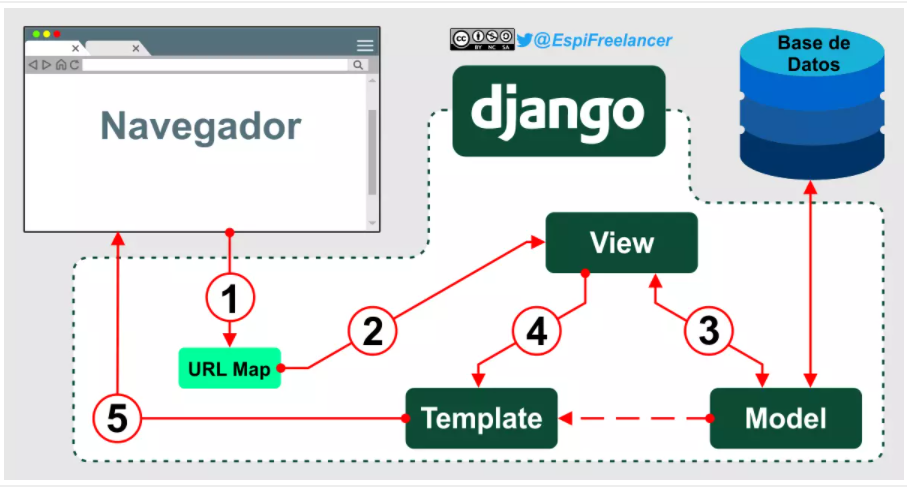
\includegraphics[scale=0.6]{MVT.png}}
  \caption{Modelo-Vista-Template}
\end{figure}

Cuando hacemos una consulta a la web, esta consulta accede al mapa de URLs, cada ruta está asociada a una vista, 
esa vista decide si necesita hacer una consulta a la base de datos, y, por tanto, irá a los modelos y después se 
mostrará la información a través de un template o directamente se muestra la información en un template.

\section{Base de datos} \label{sec:base_datos}

\subsection{Tecnología}

Para elegir que gestor de base de datos utilizar en el proyecto primero debemos pensar en qué necesidades tenemos.
Las dos características principales que deben cumplir es que sea escalable y que funcione bien en ambientes de alto volumen 
de datos ya que la aplicación comenzará a funcionar con un número pequeño de productos alimenticios pero la idea es almacenar una gran cantidad de datos.\\ \\
Mis opciones eran \textbf{PostgreSQL}, \textbf{SQLite} y \textbf{MySQL}.
SQLite era una buena opción, pero uno de sus problemas es que es difícilmente escalable y no es adecuado para grandes bases de datos.
En ese aspecto tanto PostgreSQL como MySQL son buenas opciones ya que cumplen esas características.\\ \\

Finalmente me he decidido por \textbf{PostgreSQL} debido a que MySQL es algo más compleja y se necesita cierta experiencia para configurarlo que PostgreSQL.

\subsection{Configuración}

Una vez creado nuestro proyecto de Django, por defecto nos viene configurado para usar sqlite, pero configurarlo con PostgreSQL va a ser muy sencillo.
Simplemente tenemos que instalar la librería \textbf{psycopg2} y en el archivo settings crear una base de datos que tenga el motor de PostgreSQL en lugar de sqlite3.
Además, debemos indicarle un nombre, host, credenciales de usuario y contraseña y puerto (normalmente 5432).\\ \\

Una vez hecho esto debemos crear nuestros modelos de la base de datos.

\subsection{Modelos}

He creado los modelos producto, dieta y usuario.\\
El modelo producto está formado por 23 datos que guardan información nutricional del producto como nombre, tienda, alérgenos, proteínas...

\begin{figure}[H]
  \centering
  \noindent\makebox[\textwidth]{
    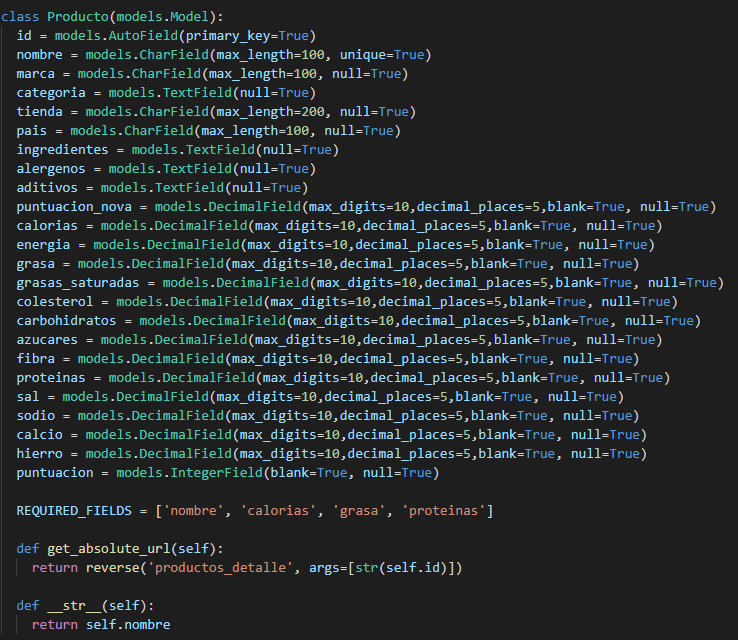
\includegraphics[scale=0.7]{productoModel.png}}
  \caption{Modelo producto}
\end{figure}

El modelo dieta está formado por un nombre, una descripción, una lista de productos y un usuario al que se le asigna.

\begin{figure}[H]
  \centering
  \noindent\makebox[\textwidth]{
    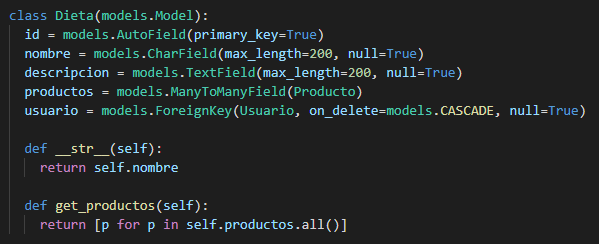
\includegraphics[scale=0.7]{dietaModel.png}}
  \caption{Modelo dieta}
\end{figure}

Para el modelo del usuario he utilizado la librería \textbf{django.contrib.auth.models} de Django, 
esta librería nos da toda la funcionalidad necesaria para crear usuarios, iniciar sesión y cerrarla. 
El problema es que sólo tiene los atributos username, password, email, nombre y apellidos.\\\\

Para solucionar esto he utilizado otra librería llamada \textbf{Base Abstract user} que te permite a partir 
de la librería anterior crear un modelo de usuario modificado con los atributos que nosotros queramos.\\

Para ello creamos el siguiente modelo de usuario, en el que tenemos atributos como peso, altura, edad, sexo y fecha de nacimiento.

\begin{figure}[H]
  \centering
  \noindent\makebox[\textwidth]{
    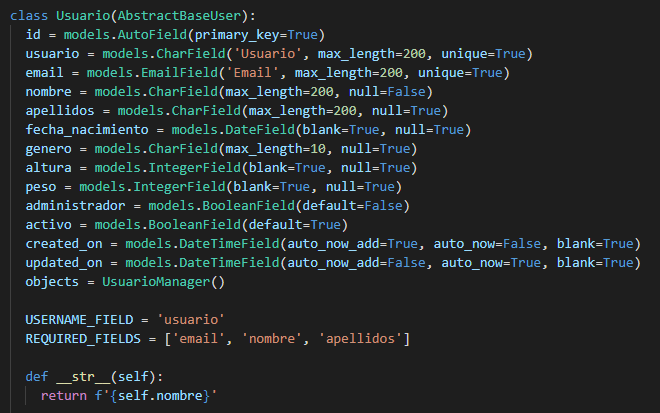
\includegraphics[scale=0.7]{usuarioModel.png}}
  \caption{Modelo usuario}
\end{figure}

Una vez tenemos el modelo de usuario simplemente en el settings indicamos dicho modelo y creamos las funciones 
para crear usuarios y súper usuarios.\\

\begin{figure}[H]
  \centering
  \noindent\makebox[\textwidth]{
    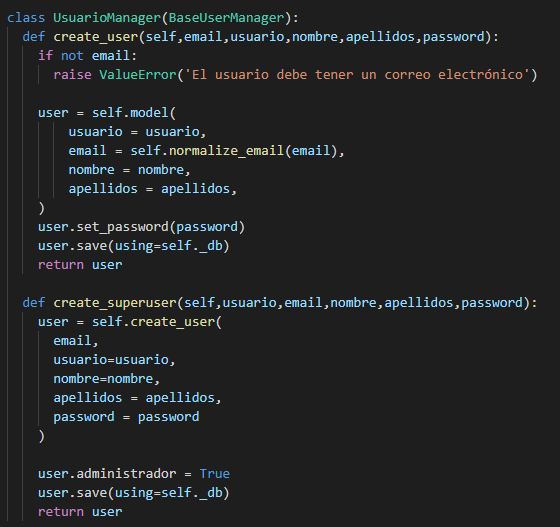
\includegraphics[scale=0.7]{usuarioManager.png}}
  \caption{Modelo usuario manager}
\end{figure}

\subsection{Formularios}

Otra parte importante serán los formularios, con estos podremos crear y modificar los modelos creados anteriormente.

\begin{figure}[H]
  \centering
  \noindent\makebox[\textwidth]{
    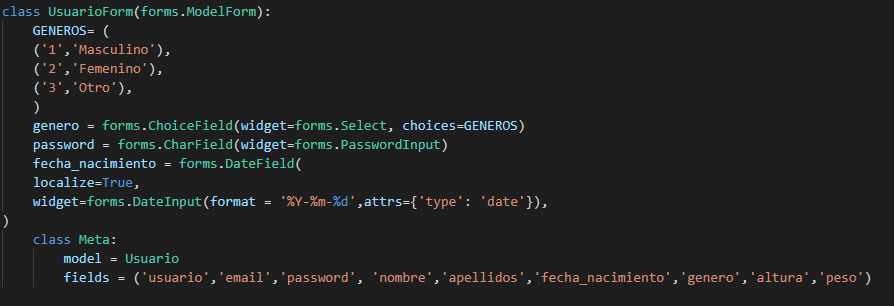
\includegraphics[scale=0.7]{usuarioForm.png}}
  \caption{Formulario de usuario}
\end{figure}

\begin{figure}[H]
  \centering
  \noindent\makebox[\textwidth]{
    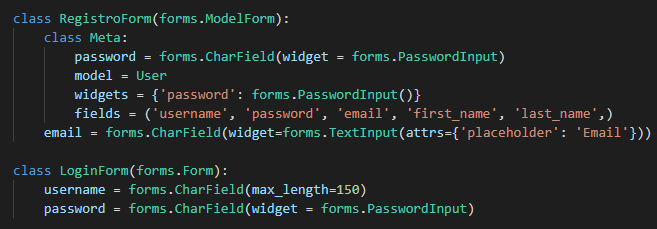
\includegraphics[scale=0.7]{registroLoginForm.png}}
  \caption{Formularios de registro y login}
\end{figure}

\subsection{Datos}

Los datos han sido descargados de la web de \textbf{Open Food Facts}, como expliqué en la sección de estado del arte \ref{sec:estado_del_arte}.
Han sido utilizados porque es una gran cantidad de productos los que contiene esa base de datos y te permite descargarlos en diferentes formatos y, muy importante,
son de código abierto.\\ \\

Una vez tenemos los datos en formato CSV, por ejemplo, procedemos a limpiar los datos. Para ello, he utilizado \textbf{Excel}. 
En cuanto a eliminar campos he hecho lo siguiente:
\begin{enumerate}
  \item He eliminado los productos cuyo nombre estuviera vacío.
  \item He eliminado valores que no fueran correctos:
  \begin{itemize}
    \item Valores calóricos que eran exageradamente grandes.
    \item Valores calóricos que eran exageradamente pequeños.
  \end{itemize}
  \item Campos que contenían caracteres especiales
\end{enumerate}

Una vez eliminados esos valores, he filtrado por productos que son procedentes de España ya que por el momento me eran suficientes.
Cuando el proyecto vaya avanzando en el desarrollo se irán incluyendo productos de otros países, pero ahora mismo la base de datos era
 demasiado grande para las herramientas que he utilizado en el despliegue \ref{sec:despliegue}.\\

\section{Frontend} \label{sec:frontend}

Para el Frontend del proyecto a desarrollar vamos a realizar una \textbf{aplicación web} ya que para los dietistas les va a ser mucho más cómodo
crear sus dietas y consultar información que, desde una aplicación móvil, y para los demás usuarios pueden consultarlo desde otros dispositivos, si así lo quisieran, 
debido a que el diseño va a ser adaptable para todo tipo de dispositivos.

Para ello, voy a utilizar \textbf{Bootstrap} \cite{bootstrap} ya que nos permite diseñar sitios webs de manera sencilla,
es de código abierto, es compatible con todos los navegadores y sus diseños son adaptables por lo que funcionan en todos los dispositivos,
además, es muy completo y presenta una gran variedad de componentes muy útiles como modales, tablas, alertas, botones...\\ \\

La idea de diseño de la web ha sido cogida de la plantilla de \textbf{AdminLTE} \cite{adminlte}. Esta plantilla es de código abierto y 
además, incluye muchos componentes útiles como la collapse-bar.

Para los iconos he utilizado la web open source \textbf{FontAwesome} \cite{iconos} que nos 
ofrece una gran cantidad de iconos gratis además de dar la capacidad de elegir el tamaño de ellos.

\section{Operaciones} \label{sec:backend}

Voy a explicar la funcionalidad de la aplicación, así como las funciones más interesantes y las bibliotecas o paquetes utilizados para ello.

Esta sería la vista principal de la web:

\begin{figure}[H]
  \centering
  \noindent\makebox[\textwidth]{
    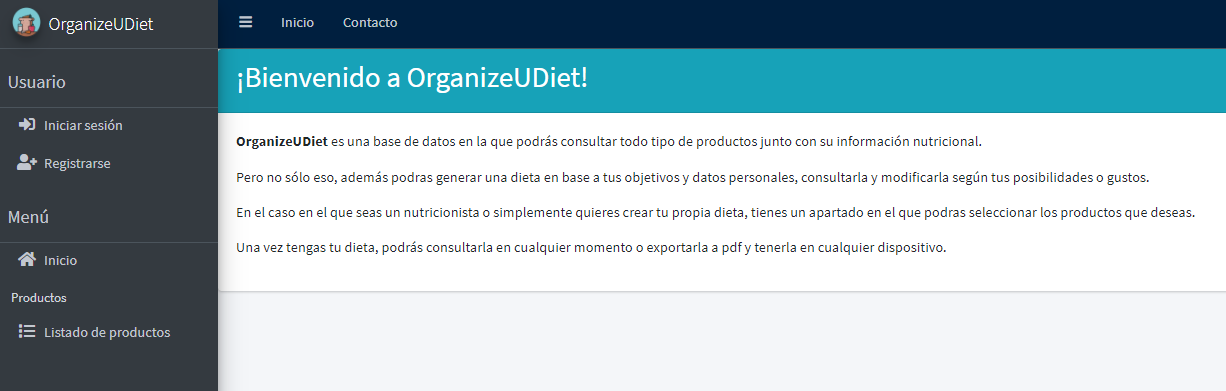
\includegraphics[scale=0.5]{index.png}}
  \caption{Página principal}
\end{figure}

Podemos iniciar sesión y registrar con formularios 

\begin{figure}[H]
  \centering
  \noindent\makebox[\textwidth]{
    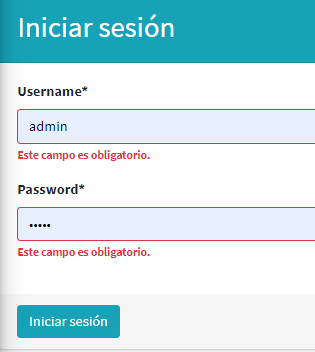
\includegraphics[scale=0.7]{login.png}}
  \caption{Vista login}
\end{figure}

\begin{figure}[H]
  \centering
  \noindent\makebox[\textwidth]{
    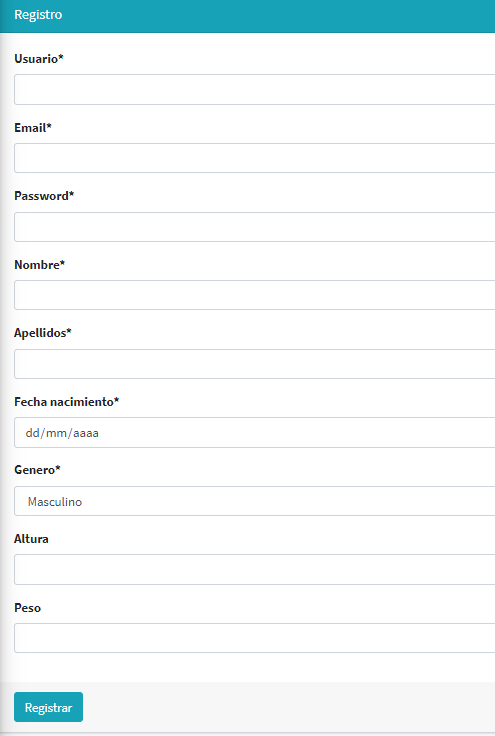
\includegraphics[scale=0.6]{registro.png}}
  \caption{Vista registro}
\end{figure}

Podemos añadir productos con un formulario con validación de datos.

\begin{figure}[H]
  \centering
  \noindent\makebox[\textwidth]{
    \includegraphics[scale=0.4]{añadirProducto.png}}
  \caption{Vista añadir producto}
\end{figure}

Visualizar el listado de productos, con enlace en el nombre para visualizarlo en detalle, con un paginador y un buscador.

\begin{figure}[H]
  \centering
  \noindent\makebox[\textwidth]{
    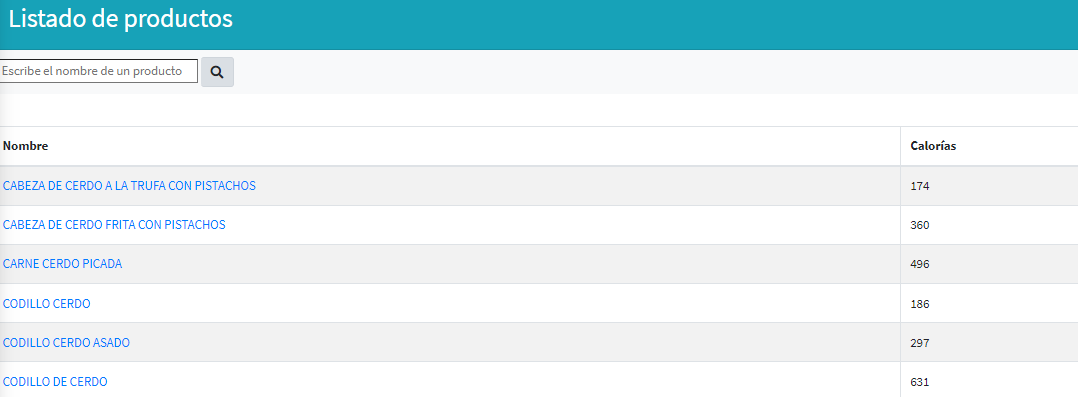
\includegraphics[scale=0.4]{listadoProductos.png}}
  \caption{Vista listado productos}
\end{figure}

\begin{figure}[H]
  \centering
  \noindent\makebox[\textwidth]{
    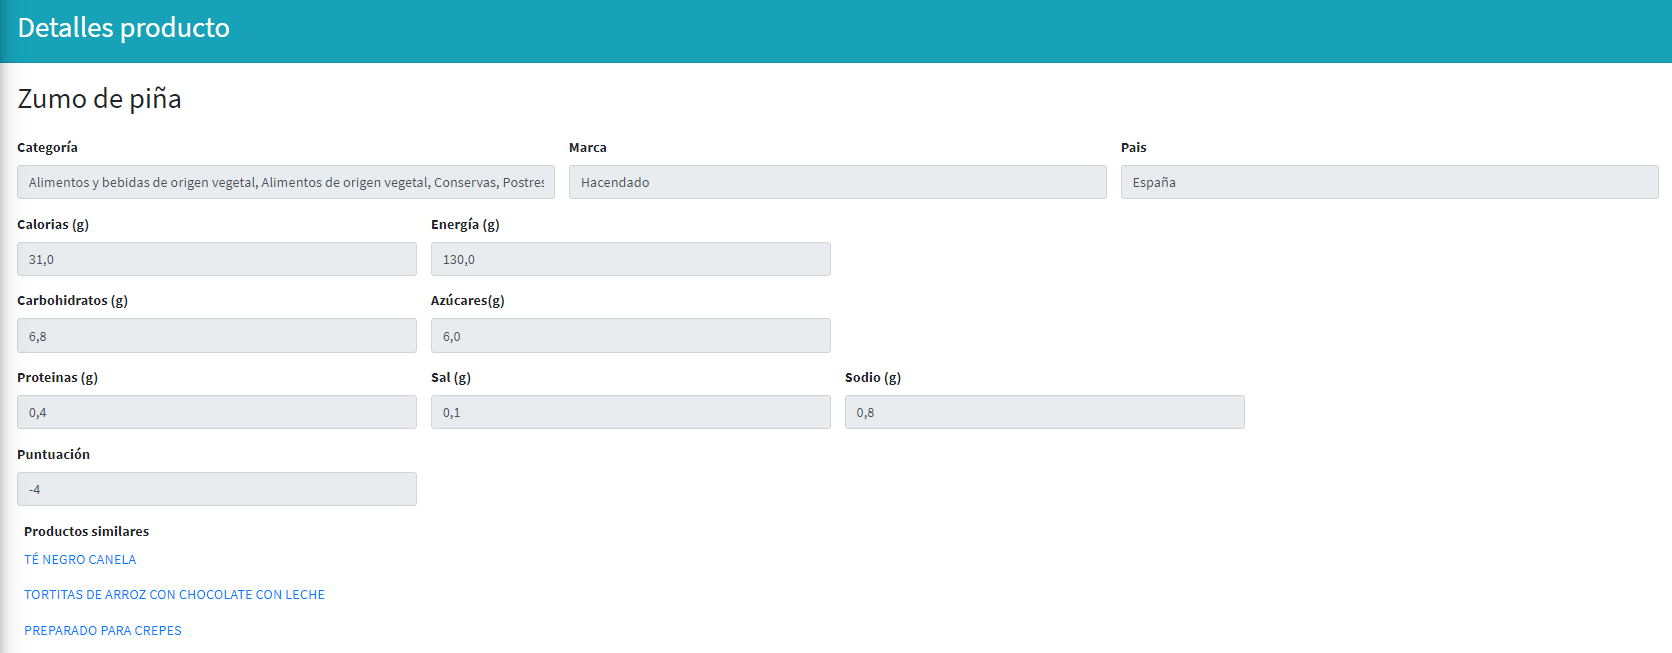
\includegraphics[scale=0.4]{consultarProducto.png}}
  \caption{Vista consultar producto}
\end{figure}

Para el paginador de la vista listado de productos he utilizado \textbf{django.core.paginator} de Django. Este paquete nos permite crear 
un paginador muy fácil simplemente llamamos a la función Paginador pasándole dos parámetros, un listado con los objetos que 
queramos mostrar y el número en el que queremos dividirlo (productos a mostrar por página):

\begin{figure}[H]
  \centering
  \noindent\makebox[\textwidth]{
    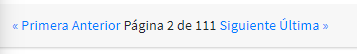
\includegraphics[scale=1]{paginador.png}}
  \caption{Paginador}
\end{figure}

Consultar nuestro perfil y modificarlo.

\begin{figure}[H]
  \centering
  \noindent\makebox[\textwidth]{
    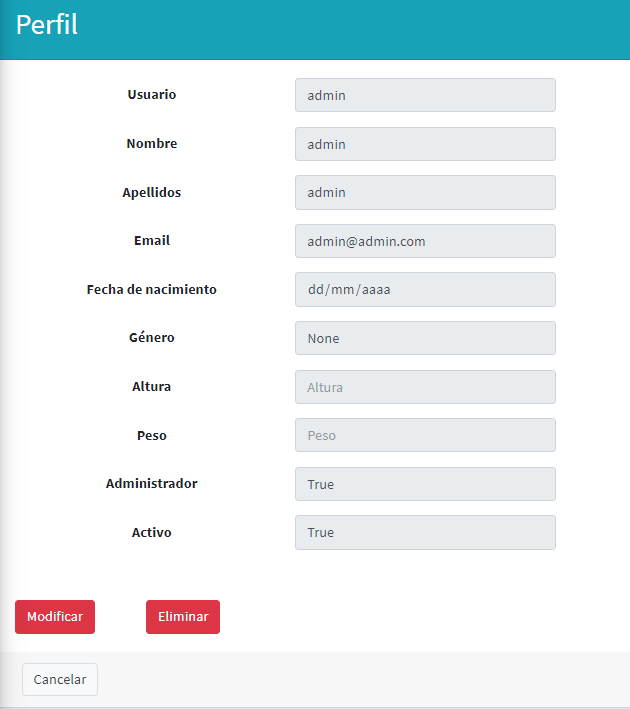
\includegraphics[scale=0.5]{consultarPerfil.png}}
  \caption{Vista consultar perfil}
\end{figure}

Para la edición y borrado de objetos como pueden ser los productos he utilizado modales de Bootstrap para confirmar la acción.

\begin{figure}[H]
  \centering
  \noindent\makebox[\textwidth]{
    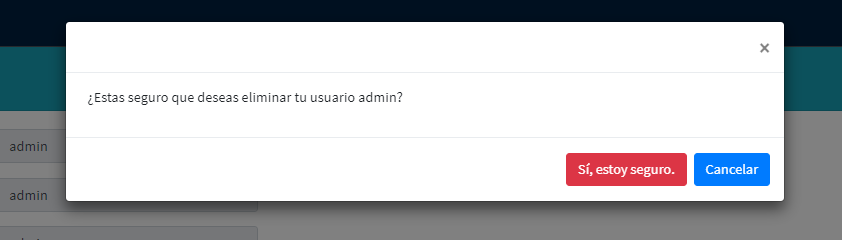
\includegraphics[scale=0.6]{modal.png}}
  \caption{Ejemplo de modal}
\end{figure}

Podemos crear una dieta seleccionando los productos que queramos y asignárnosla si somos un usuario o asignársela a otro usuario si somos un dietista.

\begin{figure}[H]
  \centering
  \noindent\makebox[\textwidth]{
    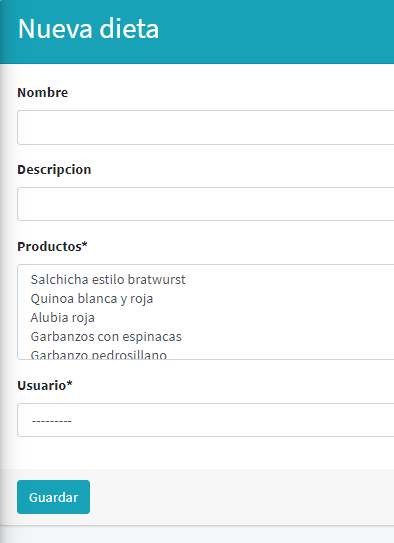
\includegraphics[scale=0.6]{crearDieta.png}}
  \caption{Vista crear dieta}
\end{figure}

\begin{figure}[H]
  \centering
  \noindent\makebox[\textwidth]{
    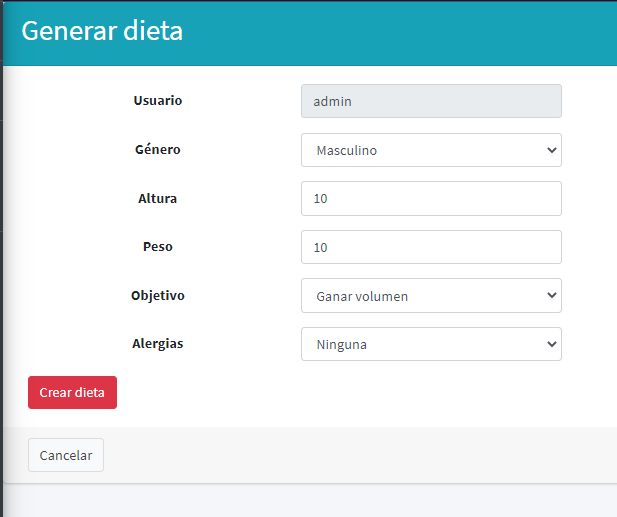
\includegraphics[scale=0.6]{generarDieta.png}}
  \caption{Formulario generar dieta}
\end{figure}

Aquí podemos ver un listado con nuestras dietas, pudiendo visualizarla en detalle o exportarla a PDF.

\begin{figure}[H]
  \centering
  \noindent\makebox[\textwidth]{
    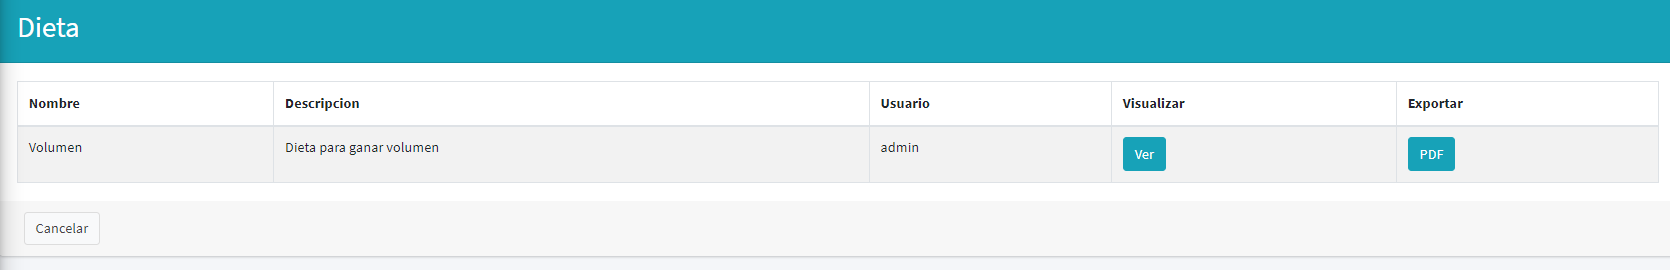
\includegraphics[scale=0.4]{mostrarDieta.png}}
  \caption{Vista mostrar dieta}
\end{figure}

%Visualziar dieta y captura
%Dieta en pdf

\newpage
\section{Tests} \label{sec:tests}

Para los tests emplearé la biblioteca \textbf{TestCase}. Es la más común en Django para la creación de test.\\
Esta biblioteca es una extensión de SimpleTestCase, pero esta sólo vale si no utilizas una base de datos 
en tu aplicación.\\

Para cada una de las funcionalidades de la web vamos a crear un test y con ella cerraremos la issue corespondiente.
Este sería un ejemplo en la que testeamos las funciones de crear y modificar un producto.

\begin{figure}[H]
  \centering
  \noindent\makebox[\textwidth]{
    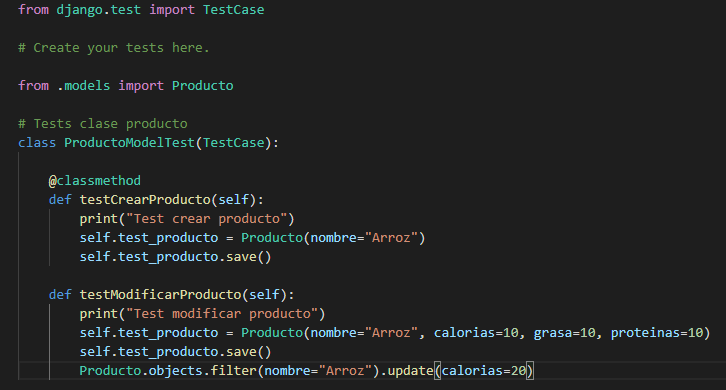
\includegraphics[scale=0.7]{test.png}}
  \caption{Test}
\end{figure}

\section{Despliegue} \label{sec:despliegue}

\subsection{Plataforma}

Por último, quedaría desplegar la aplicación, para ello voy a utilizar \textbf{Heroku}.\\

Ante las necesidades del proyecto de encontrar una plataforma de despliegue en la nube que fuera fácil de usar, pudiera actualizarse de manera automática, fuera gratuita y permitiese el lenguaje Python decidí utilizar Heroku ya que cumplía todas estas necesidades. 

\textbf{Heroku} es una plataforma en la nube que nos permite desplegar aplicaciones web en cualquier lenguaje de programación.
Además, es muy sencillo, sólo tenemos que conectar nuestro repositorio de GitHub en el que tengamos el proyecto que queremos desplegar,
podemos configurarlo para que con cada commit se haga el despliegue automáticamente y además es gratuito. Otras alternativas a Heroku 
eran Firebase y Azure.

\subsection{Librerías}

La primera librería que tenemos que instalar es \textbf{Gunicorn}. Esta librería es un servidor HTTP para Unix, sin ella nos sería imposible realizar el despliegue de nuestra aplicación.
Como en este proyecto estamos trabajando con base de datos PostgreSQL, necesitamos instalar la librería \textbf{psycopg2}. Esta librería es un adaptador a dicha base de datos para el lenguaje Python.\\\\
Heroku por defecto no permite los archivos estáticos, para solucionar este problema he incluido la librería \textbf{whitenoise}.\\
Esta librería nos permite cargar todos los archivos estáticos y se configura muy fácil, simplemente tenemos que instalarlo y en
el fichero settings.py de la aplicación incluimos el middleware y las rutas de dichos archivos que queremos cargar.\\\\
Por último, necesitamos dos librerías más, una de ellas es \textbf{dj-database-url}. Esta librería realiza la conexión entre nuestro proyecto y el gestor de base de datos de Heroku.\\
Y la otra librería es \textbf{python-decouple} para usar variables de entorno en Heroku, así evitamos poner tokens y contraseñas a la vista de todos en nuestro proyecto. \\

Por tanto, el archivo requirements.txt quedaría así:
\begin{figure}[H]
  \centering
  \noindent\makebox[\textwidth]{
    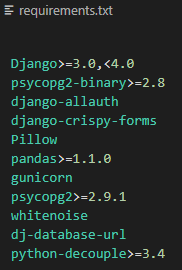
\includegraphics[scale=1]{requirements.png}}
  \caption{Archivo requirements.txt}
\end{figure}


\subsection{Configuración}

Para configurar el despliegue en Heroku como he explicado anteriormente debemos registrarnos en la web y conectar el repositorio de Github del proyecto.
Una vez hecho esto nos vamos al archivo settings.py del proyecto y hacemos lo siguiente:\\
Importamos las librerías, ponemos debug a false e incluimos en allowed\_hosts la url de despliegue o simplemente ponemos un asterisco y así acepta todas las urls.

\begin{figure}[H]
  \centering
  \noindent\makebox[\textwidth]{
    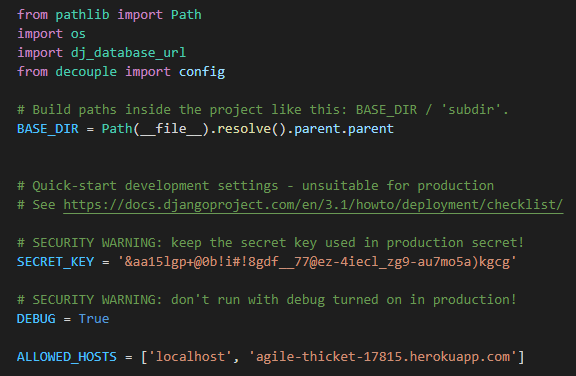
\includegraphics[scale=0.8]{settings1.png}}
  \caption{Configuración despliegue}
\end{figure}

Añadimos el middleware de whitenoise.

\begin{figure}[H]
  \centering
  \noindent\makebox[\textwidth]{
    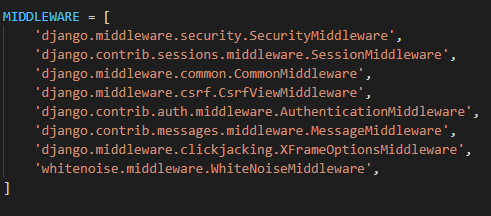
\includegraphics[scale=1]{settings2.png}}
  \caption{Configuración despliegue middleware}
\end{figure}

Indicamos la base de datos.

\begin{figure}[H]
  \centering
  \noindent\makebox[\textwidth]{
    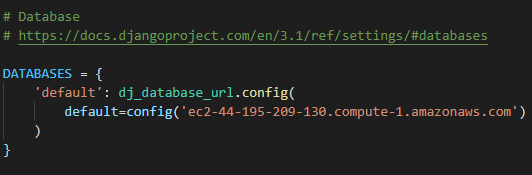
\includegraphics[scale=1]{settings3.png}}
  \caption{Configuración despliegue base de datos}
\end{figure}

Añadimos esta línea para que whitenoise cargue los archivos estáticos.

\begin{figure}[H]
  \centering
  \noindent\makebox[\textwidth]{
    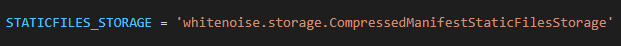
\includegraphics[scale=1]{settings4.png}}
  \caption{Configuración despliegue archivos estáticos}
\end{figure}

Ya tendríamos configurado todo. Simplemente tenemos que esperar a que se haga el despliegue si hemos configurado que se haga automáticamente con cada commit o desplegarlo nosotros desde la web.\\\\

Otra opción sería hacerlo desde local.
Nos conectamos a nuestra cuenta de Heroku con Heroku login, creamos una app de heroku con heroku create y hacemos un push desde nuestro repositorio local con:
\begin{lstlisting}
git push --prefix app keroku master
\end{lstlisting}

Conectamos nuestra base de datos con nuestra app con el siguiente comando:
\begin{lstlisting}
heroku pg:psql <nombre_bd_heroku> --app <nombre_app_heroku>
\end{lstlisting}

Ahora sólo quedaría hacer un migrate de la base de datos con:
\begin{lstlisting}
heroku run python manage.py migrate
\end{lstlisting}

Incluimos nuestros archivos sql con nuestros datos de la base de datos.
\begin{lstlisting}
heroku pg:psql --app <nombre_app> < <archivo.sql>
\end{lstlisting}
Y abrimos la aplicación con heroku open.\\\\

Para probar la aplicación aquí dejo el enlace:

\url{https://agile-thicket-17815.herokuapp.com/}